\documentclass[twoside]{article}
\setlength{\oddsidemargin}{0.25 in}
\setlength{\evensidemargin}{-0.25 in}
\setlength{\topmargin}{-0.6 in}
\setlength{\textwidth}{6.5 in}
\setlength{\textheight}{8.5 in}
\setlength{\headsep}{0.75 in}
\setlength{\parindent}{0 in}
\setlength{\parskip}{0.1 in}

%
% ADD PACKAGES here:
%
\usepackage{amsmath,amsfonts,graphicx,tikz}
\usepackage[most]{tcolorbox}
\usepackage[colorlinks=true, linkcolor=red, urlcolor=blue]{hyperref}
\usetikzlibrary{calc,arrows.meta}


\def\x0{0.6}
\pgfmathsetmacro{\ymax}{sqrt(1-(\x0)^2)}

\DeclareSymbolFont{extraup}{U}{zavm}{m}{n}
\DeclareMathSymbol{\varheart}{\mathalpha}{extraup}{86}
\DeclareMathSymbol{\vardiamond}{\mathalpha}{extraup}{87}

%
% The following commands set up the lecnum (lecture number)
% counter and make various numbering schemes work relative
% to the lecture number.
%
\newcounter{lecnum}
\renewcommand{\thepage}{\thelecnum-\arabic{page}}
\renewcommand{\thesection}{\thelecnum.\arabic{section}}
\renewcommand{\theequation}{\thelecnum.\arabic{equation}}
\renewcommand{\thefigure}{\thelecnum.\arabic{figure}}
\renewcommand{\thetable}{\thelecnum.\arabic{table}}

%
% The following macro is used to generate the header.
%
\newcommand{\lecture}[4]{
   \pagestyle{myheadings}
   \thispagestyle{plain}
   \newpage
   \setcounter{lecnum}{#1}
   \setcounter{page}{1}
   \noindent
   \begin{center}
   \framebox{
      \vbox{\vspace{2mm}
    \hbox to 6.28in { {\bf STAT 512: Statistical Inference
	\hfill Autumn 2025} }
       \vspace{4mm}
       \hbox to 6.28in { {\Large \hfill Lecture #1: #2  \hfill} }
       \vspace{2mm}
       \hbox to 6.28in { {\it Instructor: #3 \hfill Tony Lei} }
      \vspace{2mm}}
   }
   \end{center}
   \markboth{Lecture #1: #2}{Lecture #1: #2}

   \vspace*{4mm}
}

%for the motivation box
\tcbset{
  motivationstyle/.style={
    colback=gray!10!white,   % light gray background
    colframe=gray!70!black,  % darker gray border
    fonttitle=\bfseries,
    title=Motivation,
    sharp corners,
    boxrule=0.8pt,
    coltitle=black,
    enhanced
  }
}

\newenvironment{motivation}
  {\begin{tcolorbox}[motivationstyle]}
  {\end{tcolorbox}}

%Use this command for a figure
\newcommand{\fig}[3]{
			\vspace{#2}
			\begin{center}
			Figure \thelecnum.#1:~#3
			\end{center}
	}

% Red note command
\newcommand{\note}[1]{\textcolor{red}{#1}}

% Use these for theorems, lemmas, proofs, etc.
\newtheorem{theorem}{Theorem}[lecnum]
\newtheorem{lemma}[theorem]{Lemma}
\newtheorem{proposition}[theorem]{Proposition}
\newtheorem{claim}[theorem]{Claim}
\newtheorem{question}[theorem]{Question}
\newtheorem{answer}[theorem]{Answer}
\newtheorem{corollary}[theorem]{Corollary}
\newtheorem{definition}[theorem]{Definition}
\newenvironment{proof}{{\bf Proof:}}{\hfill\rule{2mm}{2mm}}

% **** ADDITIONAL MACROS:
\newcommand\E{\mathbb{E}}
\newcommand\F{\mathcal{F}}
\newcommand{\prob}{\mathbb{P}}

\begin{document}
\lecture{1}{Introduction to Probability and Statistics}{Ema Perkovic}

\section{Sample Space and Probability Measure}
First, let's recall some basic definitions of set theory and probability. 

The \textbf{sample space} ($\Omega$) is the set of all possible outcomes of a random experiment. A single outcome from the sample space is denoted as $\omega$. An \textbf{event} is a subset of the sample space, that is, $A\subseteq \Omega$. The \textbf{complement} of that event is denoted as $A^{c}$.

Let $A_i,A_j,\dots$ be events in $\Omega$. In general, we say two events are \textbf{pairwise disjoint} if  
$$A_i\cap A_j = \emptyset, \quad i\neq j.$$  
For a set $\Omega$, $A_1,\dots,A_k$ form a \textbf{partition} of $\Omega$ if  
$$\bigcup_{i=1}^kA_i = \Omega.$$
 
Now that we have the basics out of the way, let us define $\sigma$-algebras.

\subsection{$\sigma$-algebra}
\begin{motivation}
Given any subset of $\Omega$, we want to be able to define a \emph{measure} on it. Is every set measurable? Which ones are measurable? What is a measure?
\end{motivation}
\begin{definition}
    A \textbf{sigma algebra} $\mathcal{F}$ is a \textbf{collection of subsets} of $\Omega$ that satisfies:
\begin{enumerate}
  \item[(A1)] (entire/empty set) $\Omega \in \mathcal{F}$, $\emptyset \in \mathcal{F}$.
  \item[(A2)] (complement) If $A \in \mathcal{F}$, then $A^c \in \mathcal{F}$.
  \item[(A3)] (countable unions) If $A_1,A_2,\dots \in \mathcal{F}$, then $\bigcup_{i=1}^{\infty} A_i \in \mathcal{F}$.\\  
  \note{This is also true for finite unions.}\\
  \note{By De Morgan’s law, countable intersections are also in $\mathcal{F}$.}
  \end{enumerate}
\end{definition}

Now, given a pair $(\Omega,\mathcal{F})$, we say it is a \textbf{measurable space}. This means that a \textbf{measure} can be assigned to it.  
\note{Not to be confused with a \textbf{measure space}, which includes the measure itself.}

\begin{definition}
    A \textbf{measure} is a function $\mu:\mathcal{F}\rightarrow [0,\infty]$ (in general, could be signed $\mu:\mathcal{F}\rightarrow \mathbb{R}$) such that:
    \begin{itemize}
        \item $\mu(\emptyset)=0$.
        \item For any \textbf{pairwise disjoint} collection $\{A_i\}_{i=1}^{\infty}$,
        \[
            \mu\!\left(\bigcup_{i=1}^\infty A_i\right)=\sum_{i=1}^\infty \mu(A_i).
        \]
    \end{itemize}
\end{definition}

Given $\Omega$, there are many possible $\sigma$-algebras. Which one do we choose?  
The \textbf{Borel $\sigma$-algebra} on $\mathbb{R}$, denoted $\mathcal{B}(\mathbb{R})$, is the smallest $\sigma$-algebra containing all open intervals $(a,b)$ ($a,b\in\mathbb{R}$). Equivalently, it is generated by any of the families
$\{(a,b)\}$, $\{[a,b)\}$, or $\{(-\infty,a]\}$ for $a,b\in\mathbb{R}$.

We use the Borel $\sigma$-algebra because it contains all the “nice” sets we care about. In other words, it is the smallest $\sigma$-algebra that contains all the “events” that we want to measure. Now, let's define the notion of a probability

\subsection{Probabilty}
\begin{definition}
    Given a measure space $(\Omega,\mathcal{F},\mu)$, it is a \textbf{probability space} if
    $$\mu(\Omega)=1.$$ 
    In this case, $\mu$ is called a \textbf{probability measure}, denoted by $\mathbb{P}$. It must satisfy:
    \begin{itemize}
        \item [(P1)] $\prob(\Omega) = 1$.
        \item [(P2)] $\prob(A)\geq 0, \quad \forall A\in \F$.
        \item [(P3)] For any \textbf{mutually exclusive events} $\{A_i\}_{i=1}^{\infty}$,
        \[
            \prob\!\left(\bigcup_{i=1}^\infty A_i\right)=\sum_{i=1}^\infty \prob(A_i).
        \]
    \end{itemize}
\end{definition}

The axioms (P1)–(P3) imply the following:

\begin{theorem}
For any $A,B\in\mathcal{F}$,
\begin{itemize}
  \item $\mathbb{P}(\emptyset)=0$;
  \item $0\le \mathbb{P}(A)\le 1$;
  \item $A\subseteq B \ \Rightarrow\ \mathbb{P}(A)\le \mathbb{P}(B)$;
  \item $\mathbb{P}(A^{c}) = 1-\mathbb{P}(A)$;
  \item $\mathbb{P}(A\cup B)=\mathbb{P}(A)+\mathbb{P}(B)-\mathbb{P}(A\cap B)$.
\end{itemize}
\end{theorem}

From (P3), we also get the following two properties:

\begin{itemize}
    \item If $A_1\subseteq A_2\subseteq\cdots$ (an increasing sequence), then
\[
  \mathbb{P}\!\left(\bigcup_{n=1}^{\infty} A_n\right)
  = \lim_{n\to\infty}\mathbb{P}(A_n).
\]
\item If $A_1\supseteq A_2\supseteq\cdots$ (a decreasing sequence), then
\[
  \mathbb{P}\!\left(\bigcap_{n=1}^{\infty} A_n\right)
  = \lim_{n\to\infty}\mathbb{P}(A_n).
\]

\end{itemize}

Now that we have defined a notion of probability, we can consider two different views of viewing statistics. The \textbf{frequentist} view says that we can think of probability by viewing it as a \emph{frequency} observed as we repeat the experiment many times. The \textbf{Bayesian} view says that probability can be seen as a \textit{subjective} thing, where it can be updated based on your own experiences. 

\section{Random Variables}
\begin{motivation}
    When we talk about events we can easily list them out. For example, the event that we pick the 5 of clubs from a deck of cards. However, we want to deal with numbers ($\mathbb{R}$) in which case we need a function that takes in an event $A\in \Omega$ and spits out a real number.
\end{motivation}
\begin{definition}
    Let $\Omega$ be a sample space and $\F$ be a $\sigma$-algebra. A mapping $X:\Omega\rightarrow\mathbb{R}$ is a \emph{random variable} if $X(\omega)$ is measurable with respect to $\F$. More rigoursly,
    $$X^{-1}((-\infty,c]):=\{\omega\in\Omega:X(\omega\leq c)\}\in \F\qquad \forall c\in\mathbb{R}$$
\end{definition}
This means that given an interval, the inverse of $X$ would give you the set of outcomes that corresponds to that interval. For a random variable $X$, we can then define its cumulative distribution function

\begin{definition}
The CDF of a random variable $X$ is defined as
$$F(x) = P(X\leq x) = \mathbb{P}(\{\omega\in\Omega: X(\omega)\leq x\})$$
and is denoted by $F_x(x)$ or $F(x)$. This is the probability that random variable $X$ is less than some value $x$.
\end{definition}
\begin{theorem}
    The function $F(x)$ is a CDF if the following conditions hold
    \begin{itemize}
        \item [(1)]$\lim_{x\rightarrow - \infty}F(x)=0$ and $\lim_{x\rightarrow  \infty}F(x)=1$ 
        \item [(2)] $F(x)$ is a nondecreasing function of $x$
        \item [(3)] $F(x)$ is right continious, for every number $x_0$, $\lim_{x\rightarrow x_0^+}F(x)=F(x_0)$
    \end{itemize}
\end{theorem}
When $X$ only takes on discrete values, then we can characterize its distribution using the probability mass function (PMF). This is defined as 
$$p(x)=P(X=x)=F(x)-F(x^-)$$
where $F(x^-)=\lim_{\epsilon\rightarrow 0}F(x-\epsilon)$. From this notion, we can recover the CDF by $F(x)=\sum_{x'\leq x}p(x')$. This just means that we just take the sum of the discrete probabilities less than or equal to x. Then, we can extend that to the continuous case where we define the probability density funciton (PDF) as 
$$
p(x)=F'(x)=\frac{d}{dx}F(x)
$$
Thus, we can write the CDF as 
$$
F(x)=\prob(X\leq x) = \int_{-\infty}^xp(x')dx'
$$
\note{Note that the PMF and PDF are not always well-defined. This leads to the case that a random variable can have a CDF but not a PMF or PDF. Hence we like to use the CDF to characterize the random variable rather than the PMF or PDF}
\section{Common Distributions}
\subsection{Discrete Random Variables}
{\bf Bernoulli.}
If $X$ is a Bernoulli random variable with parameter $p$, 
then $X=0$ or, $1$ such that
$$
P(X=1) = p,\quad P(X=0)=1-p.
$$
In this case, we write $X\sim {\sf Ber}(p)$.

{\bf Binomial.}
If $X$ is a binomial random variable with parameter $(n,p)$, then
$X=0,1,\cdots, n$ such that
$$
P(X=k) = {n \choose k} p^k (1-p)^{n-k}.
$$
In this case, we write $X\sim {\sf Bin}(n,p)$.
Note that 
if $X_1,\cdots, X_n\sim {\sf Ber}(p)$, then
the sum $S_n = X_1+X_2+\cdots+X_n$ is a binomial random variable with parameter $(n,p)$. 


{\bf Geometric.}
If $X$ is a geometric random variable with parameter $p$, then
$$
P(X=n) = (1-p)^{n-1}p
$$
for $n=1,2,\cdots$. 
Geometric random variable can be constructed using `the number of trials of the first success occurs'. 
Consider the case we are flipping coin with a probability $p$ that we gets a head 
(this is a Bernoulli $(p)$ random variable). 
Then the number of trials we made to see the first head is a geometric random variable with parameter $p$.


{\bf Poisson.}
If $X$ is a Poisson random variable with parameter $\lambda$, then $X =0,1,2,3,\cdots$ and
$$
P(X=k)= \frac{\lambda^ke^{-\lambda}}{k!}. 
$$
In this case, we write $X\sim {\sf Poi}(\lambda)$.
Poisson is often used to model a counting process. 
For instance, the intensity of an image is commonly modeled as a Poisson random variable.

\subsection{Continuous Random Variables}

{\bf Uniform.}
If $X$ is a uniform random variable over the interval $[a,b]$, then
$$
p(x) = \frac{1}{b-a}I(a\leq x \leq b),
$$
where $I({\sf statement})$ is the indicator function such that if the ${\sf statement}$
is true, then it outputs $1$ otherwise $0$.
Namely, $p(x)$ takes value $\frac{1}{b-a}$ when $x\in[a,b]$ and $p(x)=0$ in other regions.
In this case, we write $X\sim {\sf Uni}[a,b]$.


{\bf Normal.}
If $X$ is a normal random variable with parameter $(\mu,\sigma^2)$,
then
$$
p(x) =\frac{1}{\sqrt{2\pi\sigma^2}}e^{-\frac{(x-\mu)^2}{2\sigma^2}}.
$$
In this case, we write $X\sim N(\mu,\sigma^2)$.

{\bf Exponential.}
If $X$ is an exponential random variable with parameter $\lambda$,
then $X$ takes values in $[0,\infty)$ and
$$
p(x) = \lambda e^{-\lambda x}.
$$
In this case, we write $X\sim {\sf Exp}(\lambda)$.
Note that we can also write 
$$
p(x) = \lambda e^{-\lambda x}I(x\geq 0).
$$
A \emph{double exponential} random variable $X$ is that $|X|$ is an exponential random variable. 
So its PDF will be 
$$
p(x) = \frac{\lambda}{2} e^{-\lambda|x|}.
$$



{\bf Cauchy.}
If $X\in\mathbb{R}$ is a Cauchy random variable with parameter $\mu,\sigma^2$,
then it has a PDF
$$
p(x) = \frac{1}{\pi \sigma} \frac{1}{1+(x-\mu)^2/\sigma^2}.
$$
Interesting fact: the Cauchy distribution has *no* mean (average); the parameter $\mu$ is the median.


{\bf Gamma.}
A Gamma random variable $X\geq 0$ has two parameters $\alpha,\lambda>0$
and has a PDF 
$$
p(x) = \frac{\lambda^\alpha}{\Gamma(\alpha)}x^{\alpha-1} e^{-\lambda x}I(x\geq 0).
$$
The function $\Gamma(\alpha) = \int x^{\alpha-1}e^{-x}dx$ is known as the Gamma function.

{\bf Beta.}
The Beta distribution is a continuous distribution on $[0,1]$.
So it is often used to model a ratio or a probability. 
If $X$ is a Beta random variable with parameter $\alpha,\beta$, then 
$$
p(x) = \frac{1}{B(\alpha,\beta)}x^{\alpha-1}(1-x)^{\beta-1}I(0\leq x\leq 1),
$$
where $B(\alpha,\beta) = \frac{\Gamma(\alpha)\Gamma(\beta)}{\Gamma(\alpha+\beta)}.$


{\bf Logistic.}
The logistic distribution is a random variable whose CDF follows from the logit function. 
It has two parameter $\alpha\in\mathbb{R},\beta>0$ and has a CDF
$$
F(x) = \frac{e^{\alpha+\beta x}}{1+e^{\alpha+\beta x}}  = \frac{1}{1+e^{-\alpha-\beta x}}.
$$
The PDF is 
$$
p(x) = \frac{\beta e^{-\alpha-\beta x}}{(1+e^{-\alpha-\beta x})^2} = \frac{\beta e^{\alpha+\beta x}}{(1+e^{\alpha+\beta x})^2}
$$

\section{Random Vectors}
We now define a random vector which is just a vector of random variables. I.e 
$$
\Vec{x}=(X_1,X_2,\dots,X_n)
$$

\begin{definition}
    The joint cuulative distributon function (joint CDF) of two random variables $X$ and $Y$ is defined as 
    $$F_{XY}(x,y)=\prob(X\leq x ,Y\leq y), \forall x,y$$
\end{definition}
\begin{theorem}
For random variables $X$ and $Y$ with marginal CDF $F_X(x)$ and $F_Y(y)$, the joint CDF $F_{XY}(x,y)$ satisfies the following
    \begin{itemize}
        \item [(1)] $F_x(x) = \lim_{y\rightarrow +\infty}F_{X,Y}(x,y)$ for any $x$
        \item [(2)]$F_y(y) = \lim_{x\rightarrow +\infty}F_{X,Y}(x,y)$ for any $y$
        \item [(3)] $\lim_{x,y\rightarrow +\infty}F_{X,Y}(x,y)=1$
        \item [(4)] $\lim_{x\rightarrow -\infty}F_{X,Y}(x,y)=0$ and $\lim_{y\rightarrow -\infty}F_{X,Y}(x,y)=0$ 
        \item [(5)] $\prob(x_1<X\leq x_2,y_1<Y\leq y_2)=[F_{XY}(x_2,y_2)-F_{XY}(x_1,y_2)]-[F_{XY}(x_2,y_1)+F_{XY}(x_1,y_1)]$
     \end{itemize}
\end{theorem}
When the vector is multivariate continious (both variables are continious), the joint PDF is given by 
$$p_{XY}(x,y)=\frac{\delta^2F(x,y)}{\delta x\delta y}$$
A marginal PDF can also by obtained by just integrating over the other variable
$$p_X(x)=\int_{\infty}^\infty p_{XY}(x,y)dy$$
$$p_Y(y)=\int_{\infty}^\infty p_{XY}(x,y)dx$$
When they are both discrete we just have
$$p_{XY}(x,y)= \prob(X=x,Y=y)$$
and we can sum to get the pmf for a single variable.
\note{The joint distriubtion contains information about X and Y beyond their marginals.}

\section{Conditional Probability}
Now we have a basic mathematical model for probability. 
This model also defines an interesting quantity called conditional probability. 
For two events $A,B\in\mathcal{F}$, the conditional probability of $A$ given $B$ is 
$$
\mathbb{P}(A|B) = \frac{\mathbb{P}(A\cap B)}{\mathbb{P}(B)}.
$$
Note that when $B$ is fixed, the function $\mathbb{P}(\cdot|B):\mathcal{F}\mapsto \mathbb{R}$
is another probability measure. 

\note{In general, $\mathbb{P}(A|B)\neq \mathbb{P}(B|A)$. }

{\bf Example (Exponential).}
Let $X$ be an exponential random variable with parameter $\lambda>0$
and consider two positive numbers $x,y>0$.
What is the probability $P(X>x+y|X>y)$?
In this case the two events $A = \{X>x+y\}$ (formally, $A = \{\omega: X(\omega)>x+y\}$)
and $B = \{X>y\}$. 
It is easy to see that $A\subset B$ so $A\cap B = A$.
Thus, 
\begin{align*}
P(X>x+y|X>y)  = 
\mathbb{P}(A|B) 
= \frac{\mathbb{P}(A\cap B)}{\mathbb{P}(B)}
= \frac{\mathbb{P}(A)}{\mathbb{P}(B)} = \frac{P(X>x+y)}{P(X>y)}.
\end{align*}
It is easy to see that for an exponential RV $X$, $P(X>y) = e^{-\lambda y}$,
which implies 
$$
P(X>x+y|X>y) = \frac{P(X>x+y)}{P(X>y)} = e^{-\lambda x} = P(X>x).
$$
Thus, the probability only depends on the \emph{increment} $x$, 
not $y$. 
This is known as the \emph{memoryless} property.

\section{Conditional Distribution}

For two random variables $X,Y$, the joint CDF is 
$$
P_{XY}(x,y) = F(x,y) = P(X\leq x, Y\leq y).
$$
When both variables are absolute continuous, 
the corresponding joint PDF is
$$
p_{XY}(x,y) = \frac{\partial^2F(x,y)}{\partial x\partial y}. 
$$
The \emph{conditional PDF} of $Y$ given $X=x$ is
$$
p_{Y|X}(y|x) = \frac{p_{XY}(x,y)}{p_X(x)},
$$
where $p_X(x) = \int_{-\infty}^\infty p_{XY}(x,y)dy$
is sometimes called the marginal density function. 


When both $X$ and $Y$ are discrete,
the joint PMF is 
$$
p_{XY}(x,y) = P(X= x, Y= y)
$$
and the conditional PMF of $Y$ given $X=x$ is
$$
p_{Y|X}(y|x) = \frac{p_{XY}(x,y)}{p_X(x)},
$$
where $p_X(x) = P(X=x) = \sum_{y}P(X=x,Y=y)$.

{\bf Example (triangle uniform).}
Consider  two random variables $(X,Y)$
that has a uniform PDF over the region $D = \{(x,y): x\geq 0, y\geq 0, x+y\leq 1\}$.
It is easy to see that $p(x,y) = 2$ when $(x,y)\in D$ and $0$ otherwise. 
What is the conditional PDF of $p_{Y|X}(y|x)?$\\
\begin{center}
    \begin{tikzpicture}[scale=5]
  % Axes
  \draw[->] (0,0) -- (1.1,0) node[right] {$x$};
  \draw[->] (0,0) -- (0,1.1) node[above] {$y$};
  
  % Region D: triangle
  \fill[blue!20,opacity=0.6] (0,0) -- (1,0) -- (0,1) -- cycle;
  
  % Boundary line x+y=1
  \draw[thick, red] (0,1) -- (1,0) node[midway, above right] {$x+y=1$};
  
  % Labels
  \node[below left] at (0,0) {$(0,0)$};
  \node[below] at (1,0) {$(1,0)$};
  \node[left] at (0,1) {$(0,1)$};
  
  % Shaded feasible region text
  \node at (0.3,0.3) {$D$};
\end{tikzpicture}
\end{center}

{\bf Answer:} Because the joint PDF is a constant, one can easily see that $p_{Y|X}(y|x)$
will also be a constant.
The key is to identify what is the feasible range of $y$ when $X=x$ .
We have two constraints $y\geq 0$ and $y\leq 1-x$
so the feasible range of $y$ is $[0,1-x]$.
Thus, 
$$
p_{Y|X}(y|x) = \frac{1}{1-x} I(0\leq y\leq 1-x, 0\leq x\leq 1).
    $$


{\bf Example (Beta-Bernoulli).}
Consider two random variables $X\in\{0,1\}$ and $Y\in[0,1]$ such that 
given $Y$, the random variable $X$ is a Bernoulli random variable with parameter $p=Y$. 
Namely, 
$$
P(X=1|Y) = Y,\quad P(X=0|Y) = 1-Y.
$$
Also, assume that $Y$ follows from a Beta distribution with parameter $\alpha,\beta$. 
We are interested in the conditional distribution of $Y$ given $X=x$.
%Since $X\in\{0,1\}$, it must be a Bernoulli RV. 
%What is the underlying parameter?
The conditional PDF of the Bernoulli is given as 
$$
p(x|y) = y^x(1-y)^{1-x}. 
$$
Thus, the joint PDF/PMF
$$
p(x,y) = p(x|y) p(y) = \underbrace{y^x(1-y)^{1-x}}_{\mbox{Bernoulli}} \cdot\underbrace{\frac{1}{B(\alpha,\beta)}y^{\alpha-1}(1-y)^{\beta-1}}_{\mbox{Beta}}
$$ 
We could at this point just use the definition to compute all the terms. However we can use this little trick: because $p(y|x) = \frac{p(x,y)}{p(x)}\propto p(x,y)$,
we only need to focus on the part of $p(x,y)$ that involves $y$. 
The above product shows that 
$$
p(y|x) \propto p(x,y) \propto y^{\alpha+x-1}(1-y)^{\beta-x}
$$
which is proportional to the PDF of a  Beta distribution with parameter $(\alpha' = \alpha+x, \beta' = \beta+(1-x))$. \note{This will be the constant that will normalize our probability distribution to be equal to 1}. 
Namely, when $X=1$, we will increase the $\alpha$ parameter by $1$
while keeping $\beta$ parameter the same. 
When $X=0$, we will increase $\beta$ by $1$ and keep the same $\alpha$.


The Beta-Bernoulli example illustrates the fact that the conditioning operation can be viewed 
as an information flow.
Suppose that  $Y$ is a variable of interest that is unobserved 
but it implicitly determines the distribution of $X$.
And $X$ is something that we can measure/observe (think of it as the data).
Before seeing $X$, we place a model that $Y$ is from a Beta distribution with parameter $\alpha,\beta$.
After observing $X$, this information should improve our knowledge about $Y$. 
A simple mathematical model to describe the improvement from the information is the conditional distribution. 
As is shown in the above example, the conditional distribution of $Y$ given $X$
is
a Beta distribution with parameter $\alpha+X, \beta+(1-X)$.
The change of parameter is an example of how the observed data $X$
improves our understanding of an unobserved quantity $Y$. 

\section{Independence}

Two events $A$ and $B$ are independent if 
$$
\mathbb{P}(A|B) = \mathbb{P}(A)\qquad \mbox{(or equivalently, $\mathbb{P}(A\cap B) = \mathbb{P}(A)\mathbb{P}(B)$)}.
$$
For three events $A,B,C$, we say events $A$ and $B$ are \emph{conditional independent}
given $C$  if 
$$
\mathbb{P}(A\cap B|C) = \mathbb{P}(A|C) \mathbb{P}(B|C)
$$


Extending this to random variables, $X$ and $Y$ are \emph{independent}
if the joint CDF can be factorized as
$$
F(x,y) = P(X\leq x, Y\leq y) = P(X\leq x) P(Y\leq y).
$$
When $X$ and $Y$ are {independent}, we often write $X\perp Y$.
A direct result from the factorization of CDF is that the PDF/PMF will also be factorized under independence:
$$
p(x,y) = p(x)p(y).
$$
This implies that the conditional PDF 
$$
p_{Y|X}(y|x) = \frac{p(x,y)}{p(x)} = p(y).
$$
A necessary condition for independence is that the join range of $(X,Y)$ is the cartesian product of the marginal ranges. That is to say
$$\Omega_{X\times Y}= \Omega_X \times \Omega_Y$$

Now we use the information interpretation (in the Beta-Bernoulli example) to think of the independence. 
The independence implies $p_{Y|X}(y|x)  = p(y),$
which can be interpreted that \emph{knowing $X$ does NOT change the distribution of $Y$.}
This is essentially what an intuitive meaning of independence should be--knowing the outcome of one variable does not provide any information about another variable.


When we have many random variables $X_1,\cdots, X_n$,
they are (mutually) independent if the joint CDF
$$
F(x_1,x_2,\cdots, x_n) = F(x_1)F(x_2)\cdots F(x_2),
$$
which implies
$$
p(x_1,x_2,\cdots,x_n) = p(x_1)p(x_2)\cdots p(x_n).
$$



{\bf Example (Uniform on a disk).}
Consider two random variables $X,Y$ such that they jointly follow from a distribution that is uniform over the unit disk $S_0 = \{(x,y): x^2+y^2\leq1\}$.
% \begin{center}


% \begin{tikzpicture}[scale=3]

% % ============= (a) Unit disk with conditional slice Y | X = x0 ============
% \begin{scope}
%   % Axes
%   \draw[->] (-1.15,0) -- (1.15,0) node[below right] {$x$};
%   \draw[->] (0,-1.15) -- (0,1.15) node[above left] {$y$};

%   % Fill unit disk
%   \fill[blue!15] (0,0) circle (1);

%   % Circle boundary
%   \draw[thick] (0,0) circle (1) node[above right=2pt] {$x^2+y^2=1$};

%   % Vertical slice at x = x0
%   \draw[dashed] (\x0,-1.05) -- (\x0,1.05)
%     node[below right=1pt] {$x=x_0$};

%   % Feasible Y segment on the slice
%   \draw[line width=1.2pt,red] (\x0,-\ymax) -- (\x0,\ymax)
%     node[midway,right=3pt] {$\displaystyle Y\in\big[-\sqrt{1-x_0^2},\,\sqrt{1-x_0^2}\big]$};

%   % Endpoints of feasible segment
%   \fill[red] (\x0,\ymax) circle (0.015);
%   \fill[red] (\x0,-\ymax) circle (0.015);

%   % Special-case callouts
%   \node[align=left,anchor=west] at (0.1,0.85)
%     {\small At $x_0=0$: $Y\in[-1,1]$\\[-2pt]
%      \small At $x_0=1$: $Y=0$ only};

%   % Origin label (optional)
%   \node[below left] at (0,0) {$O$};
% \end{scope}

% % ============= (b) Polar coordinates (R,Theta) on the unit disk ============
% \begin{scope}[xshift=3.0cm]
%   % Axes
%   \draw[->] (-1.15,0) -- (1.15,0) node[below right] {$x$};
%   \draw[->] (0,-1.15) -- (0,1.15) node[above left] {$y$};

%   % Fill unit disk
%   \fill[blue!15] (0,0) circle (1);

%   % Circle boundary
%   \draw[thick] (0,0) circle (1);

%   % Choose a representative point in the disk using (R,Theta)
%   % You can change these two numbers to move the point
%   \pgfmathsetmacro{\R}{0.8}
%   \pgfmathsetmacro{\Th}{38} % degrees

%   % Point P in Cartesian based on (R,Theta)
%   \path (0,0) coordinate (O);
%   \path ($(O)+(\Th:\R)$) coordinate (P);

%   % Radius vector
%   \draw[thick,->] (O) -- (P) node[midway,above right=-2pt] {$R$};

%   % Angle arc
%   \draw[very thick,->] (0.23,0) arc (0:\Th:0.23);
%   \node at ($(0.34,0)!\Th!($(0,0)+(0.34,0)$)$) {$\Theta$};

%   % Projections to show x = R cos Theta, y = R sin Theta
%   \draw[densely dashed] (P) -- ($(P)!1!(-90:(P))!(0,0)$ -| P) -- ($(P)!(0,0)!(P)$ -| P);
%   \draw[densely dashed] (P) -- ( { \R*cos(\Th) }, 0 );
%   \draw[densely dashed] (P) -- ( 0, { \R*sin(\Th) } );

%   % Tick dots and labels for projections
%   \fill ( { \R*cos(\Th) }, 0 ) circle (0.015) node[below] {$R\cos\Theta$};
%   \fill ( 0, { \R*sin(\Th) } ) circle (0.015) node[left] {$R\sin\Theta$};

%   % Mark point P
%   \fill[red] (P) circle (0.02) node[above right] {$P=(x,y)$};

%   % Helpful annotation
%   \node[align=left,anchor=west] at (-1.05,-0.95)
%     {\small Polar reparametrization:\\[-1pt]
%      \small $x=R\cos\Theta,\ y=R\sin\Theta$\\[-1pt]
%      \small $0\le R\le 1,\ -\pi<\Theta\le\pi$};
% \end{scope}

% \end{tikzpicture}
% \end{center}
Clearly, $X$ and $Y$ are not independent because when $X=0$, the feasible range of $Y$ is $[-1,1]$ while
when $X=1$, the only possible value of $Y$ is $0$. In other words, the cartesian product contains points not in the unit disk.

Now suppose we reparametrize the two random variable using polar coordinate $(R,\Theta) \in [0,1]\times [0,2\pi]$. 
Then
\begin{align*}
F(r,\theta) &= P(R\leq r, \Theta\leq\theta) {\quad \mbox{This is uniform}}\\
&  = \underbrace{\frac{1}{\pi}}_{\mbox{total area of disc}} \times \underbrace{\pi r^2\cdot \frac{\theta}{2\pi}}_{\mbox{area of sector}}\\
& = r^2 \cdot \frac{\theta}{2\pi}\\
& = F_R(r) F_\Theta(\theta),\\
F_R(r)& = r^2,\quad 0\leq r\leq 1\\
F_\Theta(\theta)& = \frac{\theta}{2\pi}, \quad 0\leq \theta\leq 2\pi.
\end{align*}
So $R\perp \Theta$, i.e., they are independent.
\note{Sometimes a change of variables can be useful for 2 variables to be independent}

{\bf Example (Independence and information).}
In the Beta-Bernoulli example, we have seen a probabilistic approach to infer an unobserved variable $Y$ 
using the information from another random variable $X$. 
That idea is something related to the so-called \emph{Bayesian inference}. 
Here we will introduce another approach to infer an unobserved quantity $\theta$ without assuming that $\theta$ is random. 
Suppose we observe $X_1,\cdots, X_n\in\{0,1\}$ that are independent.
We assume that they are all from the same Bernoulli distribution with an unknown parameter $\theta_0 = P(X_i=1)$.
In this case, we say $X_1,\cdots, X_n$ are IID (independently and identically distributed).
Given $X_1,\cdots, X_n$, how do we infer $\theta_0$? 
Under a probabilistic model, any parameter $\theta$ would implies a joint PMF
\begin{align*}
p(x_1,\cdots, x_n;\theta) = p(x_1;\theta)p(x_2;\theta)\cdots p(x_n;\theta)
\end{align*}
due to the independence. 
Since  it is a product term, we take a logarithm, which leads to 
$$
\log p(x_1,\cdots, x_n;\theta) = \log p(x_1;\theta)+\log p(x_2;\theta)+\cdots +\log p(x_n;\theta).
$$
Since $X_1,\cdots, X_n$ are observed, we can viewed the above function as a function of $\theta$,
and this function is known as the log-likelihood function
$$
\underbrace{\ell(\theta|X_1,\cdots, X_n)}_{\mbox{Total information}} = \log p(X_1,\cdots, X_n;\theta) = \sum_{i=1}^n \log p(X_i;\theta) = \sum_{i=1}^n\underbrace{\ell(\theta|X_i)}_{\mbox{Information of the $i$-th obs.}}.
$$
Informally, we can call $\ell(\theta|X_1,\cdots, X_n)$ as the total information from $X_1,\cdots, X_n$ on $\theta$. 
The independence assumption implies the above equality, which means that 
\emph{under independence, the total information is the addition of all individual information}.
In the \emph{likelihood framework}, information about $\theta$ is determined by
the log-likelihood function (Total information term). 
Note that unlike the Beta-Bernoulli example, here we did not specify any distribution of $\theta$--it is just an unknown quantity
and we use the likelihood function to infer plausible value of it. 
The famous \emph{maximal likelihood estimator} (MLE)
finds an estimated value of $\theta$ by maximizing the log-likelihood value.


\section{Total probability and Bayes theorem}
\begin{theorem}
    {\bf (Law of Total Probability)} 
If $B_1,B_2,...,B_k$ forms a partition of $\Omega$, then
$$\mathbb{P}(A) = \sum_{i=1}^k \mathbb{P}(A|B_i) \mathbb{P}(B_i).$$
In particular, we have
\begin{align*}
\mathbb{P}(A) &=\mathbb{P}(A\cap B)+\mathbb{P}(A\cap B^c)\\
\mathbb{P}(A) &= \mathbb{P}(A|B) \mathbb{P}(B) +  \mathbb{P}(A|B^c)\mathbb{P}(B^c)    
\end{align*}
\end{theorem} 
\begin{theorem}
    {\bf (Bayes rule)} This leads us to the formulation of Bayes rule.
Let $A_1,...,A_k$ be a partition of $\Omega$. If $\mathbb{P}(B)>0$ then, for $i=1,...,k$:
$$\mathbb{P}(A_i|B) =\frac{\mathbb{P}(B|A_i)\mathbb{P}(A_i)}{\underbrace{\sum_{j=1}^k \mathbb{P}(B|A_j)\mathbb{P}(A_j)}_{\mbox{By Law of Total Probability}}}.$$
\end{theorem}

We can generalize this to random variables. This gives us Bayes theorem:

\begin{theorem} {\bf (Bayes Theorem)}
    Let $X,Y$ be random variables with joint pdf $p_{xy}(x,y)$. Then Bayes Theorem states that
    \begin{eqnarray*}
p_{X|Y} (x|y) &=& \frac{p_{XY}( x,y)}{p_{Y}(y)}\\
&=& \frac{p_{Y|X}(y|x)p_X(x)}{p_Y(y)}\\
&=&\begin{cases} \frac{p_{Y|X}(y|x)p_X(x)}{\int p_{Y|X}(y|x')p_X(x')dx'}, &\quad\mbox{if $X,Y$ are absolutely continuous.}\\
\frac{p_{Y|X}(y|x)p_X(x)}{\sum_{x'} p_{Y|X}(y|x')p_X(x')}, &\quad\mbox{if $X,Y$ are discrete.}
\end{cases}
\end{eqnarray*}
\end{theorem}


{\bf Example (Poisson-Binomial). }
Consider two random variables $X$ and $Y$ such that $X\sim {\sf Poisson}(\lambda)$
and $Y|X=x$ is from a Binomial distribution with parameters $(X,p)$.
What will the marginal distribution of $Y$ be?
To study this, we attempt to compute the probability $P(Y=y).$
\begin{align*}
P(Y=y) & = \sum_xP(Y=y,X=x)\\
& = \sum_{x\geq y}P(Y=y|X=x)P(X=x)\\
&= \note{\mbox{(Note that we choose $x\geq y$ bc it doesnt make sense for $y>x$)}}\\
& = \sum_{x\geq y} {x\choose y}p^y (1-p)^{x-y}\frac{\lambda^x e^{-\lambda}}{x!}.
\end{align*}
Using the fact that ${x\choose y} = \frac{x!}{(x-y)! y!}$ and set $k=x-y$, we can rewrite the above as
\begin{align*}
P(Y=y) & = \sum_{x\geq y} {x\choose y}p^y (1-p)^{x-y}\frac{\lambda^x e^{-\lambda}}{x!}\\
&=p^ye^{-\lambda} \sum_{x\geq y}  \frac{x!}{(x-y)! y!}(1-p)^{x-y}\lambda^x \frac{1}{x!}\\
& =\frac{p^ye^{-\lambda}}{y!} \sum_{k=0}^\infty  \frac{1}{k!}(1-p)^k \lambda^{y+k}\\
& =\frac{(\lambda p)^ye^{-\lambda p}}{y!} \underbrace{\sum_{k=0}^\infty  \frac{1}{k!}(1-p)^k \lambda^{k}e^{-\lambda(1-p)}}_{=1}\\
& =\frac{(\lambda p)^ye^{-\lambda p}}{y!} \sim {\sf Poisson}(\lambda p),
\end{align*}
Thus, $Y$ follows from a Poisson distribution with parameter $\lambda p$.


\section{Conditional independence}
\begin{definition}
    {\bf (Conditional independence)} For three RVs $X,Y,$ and $Z$,
we say $X,Y$ are conditional independent given $Z$ 
if
$$
P(X\leq x,Y\leq y|Z= z) = P(X\leq x|Z=z) P(Y\leq y|Z=z)
$$
for every $x$ and $y$ 
and $z$. \note{This still includes the case that $z$ has $0$ probability}.

We use the notation
$$
X\perp Y|Z
$$
for denote the case where $X,Y$ are conditional independent given $Z$.
\end{definition}
We also have that  $X\perp Y|Z$ also implies
$$
P(X\leq x|Y=y,Z= z) = P(X\leq x|Z=z)
$$


{\bf Beware! Independence is not the same as conditional independence, i.e., $X\perp Y\not\Leftrightarrow X\perp Y|Z$. }



{\bf Example (conditional independence $\not \Rightarrow$ indepedence).}
Assume $X\perp Y|Z$ and $Z\in\{0,1\}$ such that when $Z=0$, $X$ and $Y$ are both from a uniform distribution over $[0,1]$
and when $Z=1$, $X$ and $Y$ are from a uniform distribution over $[2,3].$
Assume that $Z$ has an equal probability of being $0 $ or $1$.
Marginally, both $X$ and $Y$ are from a uniform distribution over the set $[0,1]\cup [2,3]$.
However, if we observe $X=2.5$, we know that $Y$ has to be from a uniform distribution over $[2,3]$
so $P(Y\in[0,1]|X=2.5)= 0\neq P(Y\in[0,1])=0.5$. 

The following are statements about \emph{conditional independence}

\begin{theorem}
Let $p_{XYZ}$ be the joint PDF/PMF of $X,Y,$ and $Z$.
Then the followings are equivalent:
\begin{enumerate}
\item[(i)] $X\perp Y|Z$.
\item[(ii)] $p_{XY|Z}(x,y|z)= p_{X|Z}(x|z) p_{Y|Z}(y|z)$ 
\item[(iii)] $p_{X|YZ}(x|y,z)= p_{X|Z}(x|z) $ 
\item[(iv)] $p_{XYZ}(x,y,z)= \frac{p_{XZ}(x,z)p_{YZ}(y,z)}{p_Z(z)} $ 
\item[(v)] $p_{XYZ}(x,y,z)=  g(x,z) h(y,z)$, where $g$ and $h$ are some (measurable) functions.
\item[(vi)] $p_{X|YZ}(x|y,z)=  w(x,z) $, where $w$ is some (measurable) function.
\end{enumerate}
\label{thm::cid}
\end{theorem}

Here are five important properties of conditional independence. 
Let $X,Y,Z,W$ be RVs. 
\begin{enumerate}
\item[(C1)] (symmetry) $X\perp Y|Z\Longleftrightarrow Y\perp X|Z$.
\item[(C2)] (decomposition) $X \perp Y|Z\Longrightarrow h(X)\perp Y|Z$ for any (measurable) function $h$.\\
A special case is: $(X,W) \perp Y|Z\Longrightarrow X\perp Y|Z$. 
\item[(C3)] (weak union) $X\perp Y|Z\Longrightarrow X\perp Y|Z, h(X)$ for any (measurable) function $h$.\\
A special case is: $(X,W)\perp Y|Z \Longrightarrow X\perp Y|(Z,W)$
\item[(C4)] (contraction) 
$$
X\perp Y|Z\mbox{ and } X\perp W|(Y,Z)\Longleftrightarrow X\perp (W,Y)|Z.
$$
\item[(C5)] If the joint PDF $p_{XYZW}(x,y,z,w)$ satisfies $f_{YZW}(y,z,w)>0$ almost everywhere. 
Then
$$
X\perp Y|(W,Z) \mbox{ and } X\perp W|(Y,Z) \Longleftrightarrow X\perp (W,Y)|Z.
$$
\end{enumerate}
\end{document}